\documentclass[a4paper,12pt]{article}

% Some basic packages
\usepackage[utf8]{inputenc}
\usepackage[T1]{fontenc}
\usepackage{textcomp}
\usepackage[english]{babel}
\usepackage{url}
\usepackage{graphicx}
\usepackage{float}
\usepackage{booktabs}
% \usepackage{enumitem}
\usepackage{enumerate}
\usepackage[colorlinks]{hyperref}

\pdfminorversion=7

% Don't indent paragraphs, leave some space between them
\usepackage{parskip}
\usepackage{changepage}

% Hide page number when page is empty
\usepackage{emptypage}
\usepackage{subcaption}
\usepackage{multicol}
\usepackage[dvipsnames]{xcolor}

% Other font I sometimes use.
% \usepackage{cmbright}

% Math stuff
\usepackage{amsmath, amsfonts, mathtools, amsthm, amssymb}

% Add this line to make equation numbering follow section
\numberwithin{equation}{section}

% Fancy script capitals
\usepackage{mathrsfs}
\usepackage{cancel}
% Bold math
\usepackage{bm}
% Some shortcuts
\newcommand\N{\ensuremath{\mathbb{N}}}
\newcommand\R{\ensuremath{\mathbb{R}}}
\newcommand\Z{\ensuremath{\mathbb{Z}}}
\renewcommand\O{\ensuremath{\emptyset}}
\newcommand\Q{\ensuremath{\mathbb{Q}}}
\newcommand\C{\ensuremath{\mathbb{C}}}

% Easily typeset systems of equations (French package)
\usepackage{systeme}

% Put x \to \infty below \lim
\let\svlim\lim\def\lim{\svlim\limits}

%Make implies and impliedby shorter
\let\implies\Rightarrow
\let\impliedby\Leftarrow
\let\iff\Leftrightarrow
% \let\epsilon\varepsilon

% COURSE SPECIFICS
% GRIFFITHS
\ifdefined\pdfliteral
    \let\griffPdfliteral\pdfliteral
\else \def\griffPdfliteral#1{\special{pdf: literal #1}} \fi

\newcommand\griffr[1][2]{\leavevmode\hbox{\kern1pt\vbox to1ex{}\griffPdfliteral{%
    q 1 J .27 0 0 .27 0 0 cm #1 w
    0 2 m
    0 2 8.1 9.7 9.2 13.2 c
    10.4 16.8 8.4 15.4 8 14.7 c
    7.6 14 6.8 12.6 12 13 c
    17 13.5 14.5 7.8 13.7 6 c
    12.8 4.3 10.3 1.2 11.4 .2 c
    12.6 -.7 18.8 3.6 18.8 3.6 c
    18.8 3.6 l S Q
}\kern6pt}}
\newcommand\hatgriffr{\skew3\hat{\griffr[4]}}

% Add \contra symbol to denote contradiction
\usepackage{stmaryrd} % for \lightning
\newcommand\contra{\scalebox{1.5}{$\lightning$}}

% \let\phi\varphi

% Command for short corrections
% Usage: 1+1=\correct{3}{2}

\definecolor{correct}{HTML}{009900}
\newcommand\correct[2]{\ensuremath{\:}{\color{red}{#1}}\ensuremath{\to }{\color{correct}{#2}}\ensuremath{\:}}
\newcommand\green[1]{{\color{correct}{#1}}}

% horizontal rule
\newcommand\hr{
    \noindent\rule[0.5ex]{\linewidth}{0.5pt}
}

% hide parts
\newcommand\hide[1]{}

% si unitx
\usepackage{siunitx}
\sisetup{locale = FR}

% Environments
\makeatother
% For box around Definition, Theorem, ...
% \usepackage{mdframed}
\usepackage[framemethod=TikZ]{mdframed}

% Custom command to draw a rectangular border around an equation
\setlength{\fboxsep}{5pt}  % Adjust padding inside the box
\usepackage{empheq}
\newcommand*\widefbox[1]{\fbox{\hspace{1em}#1\hspace{1em}}}

\usepackage{environ}  % This package allows for easier custom environment definitions

% Define the custom environment
\NewEnviron{framed}{%
  \begin{empheq}[box=\fbox]{align}
  \BODY
  \end{empheq}
}
% Custom environment to box align equations
% \newenvironment{boxedalign}
%   {\begin{empheq}[box=\fbox]{align}}
%   {\end{align}\end{empheq}}

\newtheorem{thm}{Theorem}[subsection]
\newtheorem{defi}[thm]{Definition}
\newtheorem{lem}[thm]{Lemma}
\newtheorem{ret}{Correction}


\newtheorem*{term}{Terminology}
\newtheorem*{key}{Keywords and Related Concepts}
\newtheorem{lign}[thm]{Equation}
\newtheorem{law}[thm]{Law / Principle}

\usepackage{mathtools}
\DeclarePairedDelimiter\bra{\langle}{\rvert}
\DeclarePairedDelimiter\ket{\lvert}{\rangle}
\DeclarePairedDelimiterX\braket[2]{\langle}{\rangle}{#1\,\delimsize\vert\,\mathopen{}#2}


% \newcounter{theo}[section]
% \renewcommand{\thetheo}{\arabic{section}.\arabic{theo}}

% \mdfsetup{skipabove=1em,skipbelow=0em}
% \theoremstyle{definition}
% \newmdtheoremenv[nobreak=true]{definition}{Definition}
% \newmdtheoremenv[nobreak=true]{theorem}{Theorem}
% \newmdtheoremenv[nobreak=true]{corollary}{Corollary}
% \newmdtheoremenv[nobreak=true]{lemma}{Lemma}

% \newtheorem*{observation}{Observation}
% \newtheorem*{property}{Property}
% \newtheorem*{postulate}{Postulate}
% \newtheorem*{conclusion}{Conlusion}
% \newtheorem*{repitition}{Repitition}
% \newtheorem*{example}{Example}
% \newtheorem*{question}{Question}
% \newtheorem*{intuition}{Intuition}

% End example and intermezzo environments with a small diamond (just like proof
% environments end with a small square)
% \usepackage{etoolbox}
% \AtEndEnvironment{example}{\null\hfill$\diamond$}%
% \AtEndEnvironment{repitition}{\null\hfill$\diamond$}%
% \AtEndEnvironment{opmerking}{\null\hfill$\diamond$}%

% Fix some spacing
% http://tex.stackexchange.com/questions/22119/how-can-i-change-the-spacing-before-theorems-with-amsthm
\makeatletter
\def\thm@space@setup{%
  \thm@preskip=\parskip \thm@postskip=0pt
}


% Exercise 
% Usage:
% \oefening{5}
% \suboefening{1}
% \suboefening{2}
% \suboefening{3}
% gives
% Oefening 5
%   Oefening 5.1
%   Oefening 5.2
%   Oefening 5.3
\newcommand{\exercise}[1]{%
    \def\@exercise{#1}%
    \subsection*{Exercise #1}
}

\newcommand{\subexercise}[1]{%
    \subsubsection*{Exercise \@exercise.#1}
}

\usepackage{xcolor}
\newcommand{\textred}[1]{\textcolor{red}{#1}}

% \lecture starts a new lecture (les in dutch)
%
% Usage:
% \lecture{1}{di 12 feb 2019 16:00}{Inleiding}
%
% This adds a section heading with the number / title of the lecture and a
% margin paragraph with the date.

% I use \dateparts here to hide the year (2019). This way, I can easily parse
% the date of each lecture unambiguously while still having a human-friendly
% short format printed to the pdf.

\usepackage{xifthen}
\def\testdateparts#1{\dateparts#1\relax}
\def\dateparts#1 #2 #3 #4 #5\relax{
    \marginpar{\small\textsf{\mbox{#1 #2 #3 #5}}}
}

\def\@lecture{}%
\newcommand{\lecture}[3]{
    \ifthenelse{\isempty{#3}}{%
        \def\@lecture{Lecture #1}%
    }{%
        \def\@lecture{Lecture #1: #3}%
    }%
    \subsection*{\@lecture}
    \marginpar{\small\textsf{\mbox{#2}}}
}

\def\@chapter{}%
\newcommand{\chapter}[3]{
    \ifthenelse{\isempty{#3}}{%
        \def\@chapter{Chapter #1}%
    }{%
        \def\@chapter{Chapter #1: #3}%
    }%
    \subsection*{\@chapter}
    \marginpar{\small\textsf{\mbox{#2}}}
}

\def\@week{}%
\newcommand{\week}[3]{
    \ifthenelse{\isempty{#3}}{%
        \def\@week{Uge #1}%
    }{%
        \def\@week{Uge #1: #3}%
    }%
    \subsection*{\@week}
    \marginpar{\small\textsf{\mbox{#2}}}
}

% These are the fancy headers
% \usepackage{fancyhdr}
% \pagestyle{fancy}

% LE: left even
% RO: right odd
% CE, CO: center even, center odd
% My name for when I print my lecture notes to use for an open book exam.
% \fancyhead[LE,RO]{Gilles Castel}

% \setlength{\headheight}{5pt}

% % \fancyhead[R]{\@lecture} % Right odd,  Left even
% \fancyfoot[R]{\thepage}  % Right odd,  Left even
% \fancyfoot[C]{\leftmark}     % Center

\makeatother

% Todonotes and inline notes in fancy boxes
\usepackage{todonotes}
\usepackage{tcolorbox}

% Make boxes breakable
\tcbuselibrary{breakable}

% Usage: 
% \begin{correction}
%     Lorem ipsum dolor sit amet, consetetur sadipscing elitr, sed diam nonumy eirmod
%     tempor invidunt ut labore et dolore magna aliquyam erat, sed diam voluptua. At
%     vero eos et accusam et justo duo dolores et ea rebum. Stet clita kasd gubergren,
%     no sea takimata sanctus est Lorem ipsum dolor sit amet.
% \end{correction}
\newenvironment{correction}{\begin{tcolorbox}[
    arc=0mm,
    colback=white,
    colframe=green!60!black,
    title=Correction,
    fonttitle=\sffamily,
    breakable
]}{\end{tcolorbox}}

% Same as 'correction' but color of box is different
\newenvironment{note}{\begin{tcolorbox}[
    arc=0mm,
    colback=white,
    colframe=white!60!black,
    title=Note,
    fonttitle=\sffamily,
    breakable
]}{\end{tcolorbox}}


% Figure support as explained in my blog post.
\usepackage{import}
\usepackage{xifthen}
\usepackage{pdfpages}
\usepackage{transparent}
\newcommand{\incfig}[1]{%
    \def\svgwidth{\columnwidth}
    \import{./figures/}{#1.pdf_tex}
}

% Fix some stuff
% %http://tex.stackexchange.com/questions/76273/multiple-pdfs-with-page-group-included-in-a-single-page-warning
\pdfsuppresswarningpagegroup=1


% My name
\author{Erik Bach Ryhl}

\graphicspath{{../figs/}}

%--------------------------
% PACKAGES
%--------------------------
\usepackage[utf8]{inputenc}
\usepackage[T1]{fontenc}
\usepackage{amsmath, amssymb, amsfonts}
\usepackage{geometry}
\usepackage{enumitem}
\usepackage{xcolor}
\usepackage{hyperref}
\usepackage{graphicx}
\usepackage{titlesec}
\usepackage{fancyhdr}
\usepackage[normalem]{ulem}

%--------------------------
% PAGE SETUP
%--------------------------
\geometry{margin=1in}
\pagestyle{fancy}
\fancyhf{}
\rhead{\thepage}
\lhead{Learning Journal}

%--------------------------
% SECTION FORMATTING
%--------------------------
\titleformat{\section}[block]{\large\bfseries}{Session \thesection:}{1em}{}
\titleformat{\subsection}[block]{\bfseries}{\thesubsection}{1em}{}
\setcounter{secnumdepth}{2}

%--------------------------
% CUSTOM ENVIRONMENTS
%--------------------------
\newenvironment{deff}[1][Definition]{\par\vspace{1em}\noindent\textbf{#1.}\hspace{0.5em}}{\par\vspace{0.1em}}

\newenvironment{rem}[1][Remark]{\par\vspace{1em}\noindent\textit{#1.}\hspace{0.5em}\begingroup\itshape}{\endgroup\par\vspace{0.1em}}

% Explanation of the custom environment:
% 1. \newenvironment{definition}[1][Definition]: This creates a new environment named "definition" with an optional argument. The default title is "Definition."
% 2. \par\vspace{1em}: Adds vertical space before the environment begins.
% 3. \noindent\textbf{#1.}: Formats the title (e.g., "Definition.") as bold text.
% 4. \hspace{0.5em}: Adds a small space between the title and the definition text.
% 5. The closing curly braces define the formatting after the environment ends, including vertical spacing.


%--------------------------
% DOCUMENT
%--------------------------
\begin{document}

\begin{center}
    {\Huge \textbf{Learning Journal}} \\
    \vspace{0.5em}
    {\large Organized by Sessions with Topic Summaries}
\end{center}
\vspace{1em}
\hrule
\vspace{2em}

%--------------------------
% TEMPLATE STRUCTURE
%--------------------------
\section*{Instructions}
\begin{itemize}
    \item Use this document to track your learning sessions.
    \item Each session entry should include: \begin{enumerate}
        \item Topics covered (briefly).
        \item Key insights or definitions.
        \item Problems attempted (with references or solutions if necessary).
        \item Questions or areas for follow-up.
    \end{enumerate}
    \textit{Make Anki flashcards of whatever makes sense. Even topics if you'd like, just to leverage their spaced repitition algorithm.}
    \item After completing a topic, write a summary essay, incorporating insights from session notes and solved examples.
\end{itemize}
\newpage

%--------------------------
% RESOURCES AND LEARNING PLANS
%--------------------------
\section*{Resources}
\subsection*{Physics}
\begin{itemize}
    \item Eigenchris
    \item MIT OpenCourseware
    \item Richard Behiel
    \item Steve Brunton
\end{itemize}
\subsection*{Math}
\begin{itemize}
    \item VisualMath on YT \begin{itemize}
        \item Lectures on quantum topology without topology seem really cool! His course notes are also free.
        \item Many overview videos
        \item Algebraic Topology
        \item Algebraic Geometry
        \item etc.
    \end{itemize}
    \item The Bright Side of Mathematics
\end{itemize}
\newpage

\section*{Learning Plan}
\textit{This is a first pass on some topics I find interesting. I don't need to understand everything the first time. I don't need to go through all the subtopics the first time. I need to understand the main idea, understand why and when it is useful, and try my hand at some basic problems to use it myself. I can always pick up these topics again since I keep a record here. Just remember to jot down your questions, the things you don't understand (and why) and what you'd like to investigate further in the future. You can \textbf{always} come back!}
\textit{The below learning plan is not set in stone. Be open for modifications and new ideas. Follow your curiosity.}
\subsection*{Calculus of Variations in Physics - \textred{21th December}}   
\begin{itemize}
    \item \sout{Understand the derivation of the Euler-Lagrange Equations}
    \item Solve the QM problem in Hand and Finch (17th December)
    \item Answer questions below and synthesize and finalize notes on the topic (20th December)
\end{itemize}
\textbf{Questions}
\begin{itemize}
    \item How is it used in modern physics today?
    \item Does one use different "actions" when working on separate problems. If so, could one find a problem "midway" between those problems and see what the action looks like there? Maybe smoothly interpolate an action between these two problems to gain a deeper understanding of how and why they need different descriptions. Maybe find a general description which they are both special cases of. 
\end{itemize} 
\subsection*{Special Relativity, Classical Field Theory and Tensors - 28th December}
\begin{itemize}
    \item Susskind Book (26rd December)
    \item Learn some tensor notation from Tong Notes
    \item Solving some basic problems with 4-vectors (27th December)
    \item Synthesize and finalise (28th December)
\end{itemize}
\subsection*{Floquet Theory - 31st December}
\subsection*{Schuller's Course and self-defined problems - 31st Janurary}
\subsection*{Linear Algebra Refresher - 7th February}
\subsection*{Complex Analysis Basics - 14th February}
\subsection*{MIT Quantum Mechanics Course - 7th February}
\subsection*{Misc. things}
\begin{itemize}
    \item Green's Function solution of Poisson's equation to get the electric potential from Griffiths
\end{itemize}
\newpage

%--------------------------
% SESSIONS
%--------------------------
\section{Session Date: 3rd January, 2025}
\subsection*{Main Topic: Electromagnetism}
\subsection*{Topics Covered: Ch. 10 Griffiths}
\begin{itemize}
    \item Solution to the four-dimensional wave-equation
    \item Liénard-Wiechert potentials
    \item Fields from a moving point charge
\end{itemize}

\subsection*{Notes}
\subsubsection*{Idea: Potential Formulation of Electrodynamics}
The goal of Chapter 10 in Griffiths is to find a general solution to Maxwell's equations in terms of potentials (we are working in the Lorenz Gauge). The very central thing to keep in mind is that information travels at the speed of light, such that the potential at some distance \(\griffr[2]\) isn't given by the source distributions at some time \(t\), but rather at the retarded time (dependent on the distance to the source) \begin{align*}
    \boxed{t_r = t - \frac{\griffr[2] }{c}}\tag{10.25}
\end{align*}

By finding the solution to Maxwell's equations in the potential formulation 
\begin{align*}
    &\square^{2} V(\mathbf{r}, t) = - \frac{1}{\epsilon _0} \rho (\mathbf{r}, t)\\
    &\square^{2} \mathbf{A}(\mathbf{r}, t) = -\mu _0 \mathbf{J}(\mathbf{r}, t)
\end{align*}
we can subsequently calculate the fields. But since the relevant \textit{time} now depends on position (space-time), differentiating sources is non-trivial. And this even applies to point charges. This is because classical electrodynamics formulates sources in terms of densities, and as such we have to define the densities related to point charges as the density of a charge with finite extension as the size goes to zero. It seems weird that there can be different retarded times from the same field point to a point charge, but that's apparently necessary with classical electrodynamics. 

\subsubsection*{The Generalized Potentials}
We have already found solutions for electro\textit{statics} (with the Coloumb Gauge) \begin{align*}
    V(\mathbf{r}) &= \frac{1}{4\pi\epsilon_0} \int \frac{\rho (\mathbf{r}^{\prime} )}{\griffr[2] } d \tau ^{\prime}\\
    \mathbf{A}(\mathbf{r}) &= \frac{\mu_0}{4 \pi } \int \frac{\mathbf{J}(\mathbf{r}^{\prime} )}{\griffr[2]} d \tau ^{\prime} 
\end{align*}
The naïve idea is to just make the transition \begin{align*}
    &\rho (\mathbf{r}^{\prime} ) \to \rho (\mathbf{r}^{\prime}, t)\\
    &\mathbf{J}(\mathbf{r}^{\prime} ) \to \mathbf{J}(\mathbf{r}^{\prime}, t)
\end{align*}
BUT, since the fields can maximally communicate at the speed of light, the sources should not be evaluated at some global time \(t\), but rather we should evaluate them at the \textit{retarded} time:
\begin{align*}
    t_r = t - \frac{\griffr[2] }{c}
\end{align*} 
which means that any field point "sees" the charge distribution at a different time depending on the radial distance from the source (and as such there are in fact infinitely many retarded times, dependent on the relative distance). It turns out that the generalisation of Maxwell's equations in terms of retarded potentials in fact is just the naïve potentials, but with the retarded times instead \begin{align*}
    \boxed{V(\mathbf{r}, t) = \frac{1}{4\pi\epsilon_0} \int \frac{\rho (\mathbf{r}^{\prime}, t_r )}{\griffr[2] } d \tau ^{\prime}, \qquad \mathbf{A}(\mathbf{r}, t) = \frac{\mu_0}{4 \pi } \int \frac{\mathbf{J}(\mathbf{r}^{\prime}, t_r)}{\griffr[2]} d \tau ^{\prime}} \tag{10.26}
\end{align*}
Notice how we on the left have find the potential at the point \(\mathbf{r}\) at the time \(t\), whereas we on the right have the source point \(\mathbf{r}^{\prime} \)  and the retarded time \(t_r\). But since this is integrated away, we end up with the correct dependencies. Since every field point sees the source point at a distinct retarded time (depending on radial distance) it does not seem so out of touch to think about \((\mathbf{r}^{\prime}, t_r)\) as a coordinate in 4 dimensions without making the time coordinate too special. We can already see how a "native relativistic" formulation of these equations could be quite elegant.

This can directly be showed to solve Maxwell's equations \begin{align*}
    &\square^{2} V(\mathbf{r}, t) = - \frac{1}{\epsilon _0} \rho (\mathbf{r}, t)\\
    &\square^{2} \mathbf{A}(\mathbf{r}, t) = -\mu _0 \mathbf{J}(\mathbf{r}, t)
\end{align*}
just by taking the gradient and then the divergence. 
\subsubsection*{Mathematical Takeaways}
\paragraph{Remember the chain rule!}
Some takeaways from that derivation is \begin{align*}
    \nabla \left( \frac{\rho (\mathbf{r}^{\prime} , t_r)}{\griffr[2] } \right) &= \partial  _i \left( \frac{\rho (\mathbf{r}, t_r)}{\griffr[2] } \right)\\
    &= \frac{1}{\griffr[2] }\partial  _i \rho + \rho \partial_i \left( \frac{1}{\griffr[2] } \right) \\
    &= \frac{1}{\griffr[2] }\frac{\partial \rho}{\partial t} \frac{\partial t}{\partial t_r} \frac{\partial t_r}{\partial x_{i} }  - \rho \frac{\hatgriffr }{\griffr[2] ^{2} } \\
\end{align*}
and since \begin{align*}
    \partial _{t_r} t = 1
\end{align*}
we get that \begin{align*}
    \nabla \left( \frac{\rho (\mathbf{r}^{\prime} , t_r)}{\griffr[2] } \right) &= -\frac{1}{c \griffr[2] }\dot{\rho} \partial _i \griffr[2] - \rho \frac{\hatgriffr }{\griffr[2] ^{2} }\\
    &= -\frac{1}{c} \dot{\rho }\frac{\hatgriffr }{\griffr[2] } -  \rho \frac{\hatgriffr }{\griffr[2] ^{2} }
\end{align*}
\paragraph{Component Form and Free Indicies are your Best Friends}
Use "dimensional analysis" with free indicies. A gradient is a vector for example. Thus when we look at the above derivation, we see that we have a vector on the left hand side. Therefore every term on the right hand side \textit{needs} to have one - and only one - free index. When taking the divergence we get a scalar because we have an index contraction, and thus every term should be of the form \(\left[   \left( \cdot  \right)_i \left( \cdot  \right)_i\right]\) - thus \textit{zero} free indicies. The advantage of writing every thing out in components allows us to use the usual product and Leibniz rules for differentation and we just have to respect indicies. 

In showing that the retarded potentials given here are indeed correct, one uses that \begin{align*}
    &\nabla \left( \frac{1}{\griffr[2] } \right) = - \frac{\hatgriffr }{\griffr[2] ^{2} }\\
    &\nabla \griffr[2] = \hatgriffr \\
    &\nabla \cdot \left( \frac{\hatgriffr }{\griffr[2] } \right) = \frac{1}{\griffr[2] ^{2} }\\
    &\nabla \cdot \left( \frac{\hatgriffr }{\griffr[2] ^{2} } \right) = 4 \pi \delta^3 (\hatgriffr )
\end{align*}

\paragraph{Coordinate Free Expressions}
It is often the case that we analyse some geometrical problem in the plane or in 3D using a specific coordinate system and specific angles. After having found expressions for certain quantities, see if you can write them in a coordinate free form - this means writing it in terms of dot products or cross products between vectors. This is a very powerful (and natural) way to generalize formulas, since there is nothing special about the coordinate systems we use other than the fact that axes are orthonormal. A simple example is the drawing from page 458 in Griffiths, where we use the unit vector \(\hatgriffr \) to write the cosine of the angle in a coordinate free form:
\begin{align*}
    v \cos \theta = \hatgriffr \cdot \mathbf{v}
\end{align*} 

Regarding this, notice the cool coordinate free from using the above ideas (\(\mathbf{A}\) and \(\mathbf{B}\) are vector fields dependent on position): \begin{align*}
    \left[  \nabla (\mathbf{A}\cdot \mathbf{B}) \right]_i = \partial _i \left( A_j B_j \right) = B_j \partial _i A_j + A_j \partial _i B_j = \left[\mathbf{J}_\mathbf{A}(\mathbf{r}) \mathbf{B} + \mathbf{J}_\mathbf{B}(\mathbf{r}) \mathbf{A}\right]_i
\end{align*}
where \(\mathbf{J}_\mathbf{A}(\mathbf{r})\) denotes the Jacobian of the vector field \(\mathbf{A}\) with respect to the cartesian axes. The Jacobian is a matrix (2 free indicies) and the \(i\)'th element is thus \begin{align*}
    \left[ \mathbf{J}_\mathbf{A}(\mathbf{r})\mathbf{B} \right] _i = \left[ \mathbf{J}_\mathbf{A}(\mathbf{r}) \right]_{ij} B_j
\end{align*} 
where Einstein summation is still implied.

Note especially that this is how a Jacobian is denoted in component form: \(\partial _i A_j\).

\subsubsection*{Liénard-Wichart Potentials: Geometrical Derivation}
\subsubsection*{Liénard-Wichart Potentials: Dirac-Delta Proof}
\subsection*{Problems Attempted}
\paragraph{Problem 10.12 in Griffiths}
\begin{figure}[h]
    \centering
    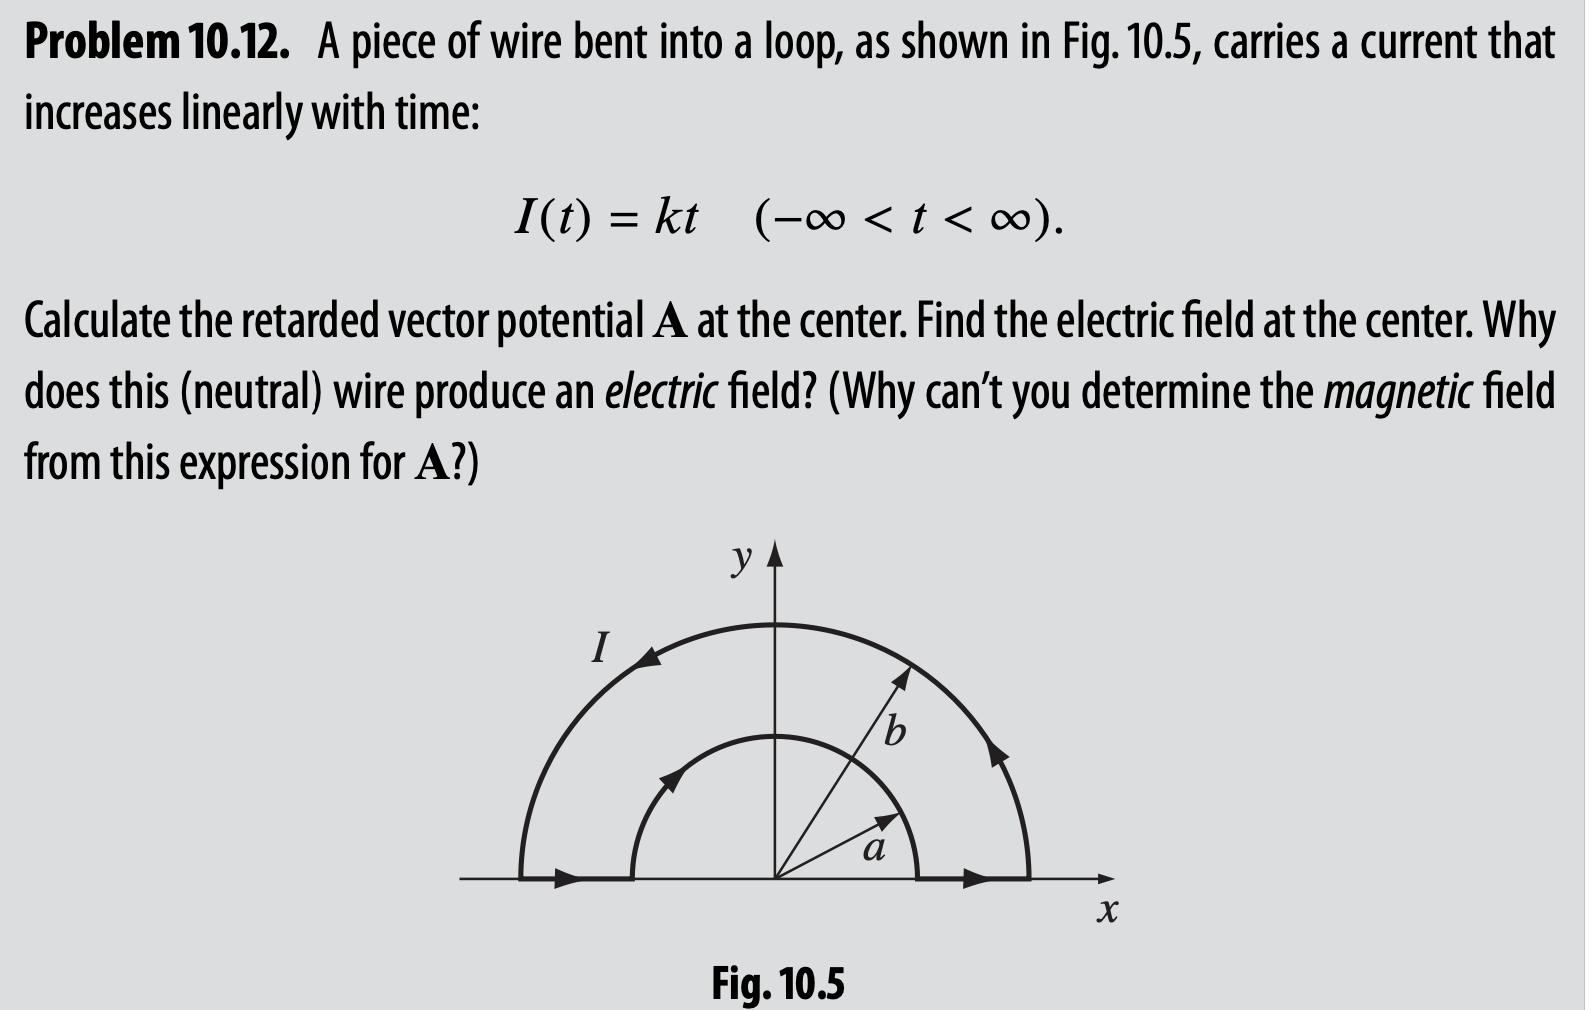
\includegraphics[width=0.8\textwidth]{Griffiths_prob_10_12.png}
\end{figure}

In general, the relevant one-dimensional integral is along the wire: \begin{align*}
    \mathbf{A}(\mathbf{r}, t) = \frac{\mu_0}{4 \pi } \int \frac{\mathbf{I}(\mathbf{r}^{\prime} , t_r)}{\griffr[2] } d l ^{\prime} 
\end{align*}

But the current only depends on time and not on position. Along the top wire we get \begin{align*}
    \mathbf{I}(t_r) = k(t - \frac{b}{c})\hat{\boldsymbol{\phi}} = (t - \frac{b}{c})\left[ - \sin \theta \hat{\mathbf{x}} + \cos \theta \hat{\mathbf{y}} \right] 
\end{align*}
while along the bottom we have \begin{align*}
    \mathbf{I}(t_r) = k(t - \frac{a}{c})(-\hat{\boldsymbol{\phi}}) = (t - \frac{a}{c})\left[ \sin \theta \hat{\mathbf{x}} - \cos \theta \hat{\mathbf{y}} \right] 
\end{align*}
such that from those contributions we get \begin{align*}
    \mathbf{A}_{\text{top and bottom}}(\mathbf{r}, t) = \frac{k\mu_0}{4 \pi } \biggl[ &\hat{\mathbf{x}} \int_0 ^\pi  d \theta \sin \theta \left( a\left( t- \frac{a}{c} \right) +  b\left(t - \frac{b}{c}\right) \right)\\
      &\hat{\mathbf{y}} \int_0 ^\pi d \theta \cos \theta \left( b \left( t - \frac{b}{c} \right) + a \left( t - \frac{a}{c} \right)   \right) \biggr]
\end{align*}
plenty of things are independent of \(\theta \) so we get \begin{align*}
    \mathbf{A}_{\text{top and bottom}}(\mathbf{r}, t) = \frac{k\mu_0}{2\pi } \left( t (a + b) -  \frac{1}{c}\left( a^{2} + b^{2}  \right) \right) 
\end{align*}
whereas from the horizontal segments we get (I think they will be equal, but the "doppler" effect would actually play in here with a point charge. This is why we have terms involving the velocity vector in that case. But here I think they should be the same in the sense that it is symmetrical w.r.t.\ time):
\begin{align*}
    \mathbf{A}_{\text{left horizontal}}(\mathbf{r}, t) &= \frac{k\mu_0}{4 \pi } \hat{\mathbf{x}} \int_b ^a \frac{t - \frac{x^{\prime}}{c} }{x^{\prime}} dx^{\prime} \\
    &=  \frac{k\mu_0}{4 \pi } \hat{\mathbf{x}} \left( t \ln \left(\frac{a}{b}\right) - \frac{a - b}{c} \right) 
\end{align*}
but of course with the right horizontal, we are integrating the exact same thing, but from \(a \to  b\). Thus they cancel. This seems wierd to me right now, since with the right hand rule from the current, I would think the field would have to contribute something. But I do see that the center is on the line of the two horizontal segments. But if we only had one side, that should prevent the field, right? I got a contribution from the left side alone. It was just cancelled by the right side it seems.  

\subsection*{Follow-Up Questions/Ideas/ToDos}
\begin{itemize}
    \item It seems weird that there can be different retarded times from the same field point to a point charge, but that's apparently necessary with classical electrodynamics. \textred{What's the full story?}
    \item In problem 10.12 above, it confuses me that flipping the limits of integration is the same as flipping the direction of the current in some sense. When we are running along the inner half circle (the one at radius \(a\)), I have the urge to say that it is running in the direction \(- \boldsymbol{\hat{\mathbf{\phi}}}\) while the angle being sweeped is from \(\pi \to 0\). But this is "a double flip" and leaves the integral unchanged. At the same time, I feel like the two horizontal wire segments shouldn't cancel. They are running in the same direction one would think. But with respect to the center point, they \textit{are} running in oppositse directions of course.  
\end{itemize}

\newpage
\section{Session Date: 4th of January, 2025}
\subsection*{Main Topic: Electromagnetism}
\subsection*{Topics Covered}
\begin{itemize}
    \item Liénard-Wiechert Potentials Continued
\end{itemize}

\subsection*{Key Insights}
\textit{Write down definitions, theorems, or takeaways. Use this space for concise notes.}

\subsection*{Problems Attempted}
\paragraph{Derivation of the Liénard-Wiechert Potentials}
\begin{align*}
    V(\mathbf{r}, t) = \frac{1}{4\pi\epsilon_0} \int \frac{\rho(\mathbf{r}^{\prime}, t_r)}{\griffr[2] (t_r)} d \tau ^{\prime} 
\end{align*}
Since \begin{align*}
    t_r = t - \frac{\griffr[2] (t_r) }{c} = t - \frac{\left| \mathbf{r} - \mathbf{w}(t_r)\right|}{c}
\end{align*}
we have that \begin{align*}
    \griffr[2] (t_r) = \left| \mathbf{r} - \mathbf{w}(t_r)\right| = c (t - t_r)
\end{align*}
where \(\mathbf{w}(t_r)\) is the trajectory of the particle, evaluated at the retarded time (since this is the reality that any different point in space-time sees!).

We also have that \begin{align*}
    \rho(\mathbf{r}^{\prime} , t_r) = q \delta ^3(\mathbf{r}^{\prime} - \mathbf{w}(t_r))
\end{align*}
This can be read as "Any observer will see a point charge \(q\) not at the position \(r^{\prime} \)  \(\mathbf{w}(t)\) at the current time \(t\), but instead at the position \(\mathbf{w}(t_r)\) which is where the particle was a while ago, at the time \(t_r\)". Remember that we are integrating over the primed coordinates.

In fact this is our regular expression for a point charge just in terms of retarded times since \begin{align*}
    \mathbf{r}^{\prime} - \mathbf{w}(t_r) = \griffr[4] 
\end{align*}

Thus I would think that our expression would be \begin{align*}
    V(\mathbf{r},t) = \frac{q}{4\pi\epsilon_0} \int \frac{\delta ^3 (\mathbf{r}^{\prime} - \mathbf{w}(t_r))}{\left| \mathbf{r} - \mathbf{w}(t_r) \right| } d \tau ^{\prime} 
\end{align*}

But my lecture notes does as following: Introduces another integration step, changes integration variable AND has a different denominator (which functional dependence I am not sure of) without a different numerator:
\begin{align*}
    V(\mathbf{r}, t) = \frac{q}{4\pi\epsilon_0} \int d \mathbf{r}^{\prime}  \int dt \frac{\delta ^3 (\mathbf{r}^{\prime} - \mathbf{w}(t))}{\left| \mathbf{r} - \mathbf{r}^{\prime}  \right| } \delta(t - t_r)
\end{align*}
I can see how performing the \(d \mathbf{r}^{\prime} \) integral would give the same denominator, but now the integral is suddenly very different. It is over time and the numerator is a delta function involing \(t\) and \(t_r\). Could you explain everything that is happening here for me? I would really like to master these types of integral transforms and \textit{wield} them so I am more comfortable with doing something like this in the future by myself.   


Now, here comes an interesting step, which I don't quite understand. We introduce another integration while integrating over \(\mathbf{r}^{\prime} \) instead of \(d \tau ^{\prime} \): \begin{align*}
    V(\mathbf{r}, t) = \frac{q}{4\pi\epsilon_0} \int d \mathbf{r}^{\prime}  \int dt \frac{\delta ^3 (\mathbf{r}^{\prime} - \mathbf{w}(t))}{\left| \mathbf{r} - \mathbf{w}(t)  \right| } \delta(t - t_r)
\end{align*}

\subsection*{Follow-Up Questions/Ideas/ToDos}
\begin{itemize}
    \item \textit{Write down any gaps in understanding or questions to revisit.}
\end{itemize}

\newpage
\section{Session Date: 5th of January, 2025}
\subsection*{Main Topic: Electromagnetism}
\subsection*{Topics Covered}
\begin{itemize}
    \item Liénard-Wiechert Potentials
\end{itemize}

\subsection*{Key Insights}
\textit{Write down definitions, theorems, or takeaways. Use this space for concise notes.}
\paragraph{Clarification of integration techniques} When we write the integral \begin{align*}
    V(\mathbf{r}, t) = \frac{1}{4\pi\epsilon_0} \int \frac{\rho (\mathbf{r}^{\prime}, t_r)}{\left| \mathbf{r} - \mathbf{r}^{\prime}  \right| } d \tau ^{\prime} 
\end{align*}
we have to be very clear about what we are calculating. First of all, We are integrating over a fixed, stationary \textit{volume} in space. This is why no time dependence is implied in the denominator. Every point in the volume we are integrating over will have a static distance to the field point \(\left| \mathbf{r} - \mathbf{r}^{\prime} \right| \). Secondly, writing \(d \tau ^{\prime} \) is the same as writing \(d^3 r\) or even \(d \mathbf{r}\). So the integration variable didn't change in the above derivation. It was just another notation. Third, even though the integration \textit{region} is fixed and independent of time, the \textit{density} of charge at that point is not. And \emph{this} is what we wish to evaluate at the retarded time, \(t_r\). But the retarded time depends on the distance from the source point to the field point \begin{align*}
    t_r = t - \frac{\left| \mathbf{r} - \mathbf{r}^{\prime}\right| }{c}
\end{align*} 

And here comes the integral trick being used above: Instead of having to remember that we should evaluate our charge distribution at the retarded time (an implicit dependence \(\rho (\mathbf{r}, t_r)\) ), which depends on the primed coordinates which we are integrating over, making the whole thing quite convoluted, we can instead integrate over \textit{all} time, and just use a delta function to pick out the retarded time only and thus make the dependence excplicit mathematically (\(\delta (t^{\prime}  - t_r)\) ). This separates time and space as integration variables formally, so to say. And if our functions are nice enough (which they often are in physics), this subsequently allows us to carry out first the (independent) space integral and \textit{then} the time integral (we are really using the Green's functions solution to the wave equation here), while the dependencies are being "managed" explicitly by the delta functions: \begin{align*}
    V(\mathbf{r}, t) &= \frac{1}{4\pi\epsilon_0} \int \frac{\rho (\mathbf{r}^{\prime} , t_r)}{\left| \mathbf{r} - \mathbf{r}^{\prime} \right| } d^3 r^{\prime} \\
    &= \frac{1}{4\pi\epsilon_0} \int d^3r^{\prime}  \int_{-\infty}^{\infty} dt^{\prime} \frac{\rho (\mathbf{r}^{\prime} , t^{\prime} )}{\left| \mathbf{r} - \mathbf{r}^{\prime}  \right| } \delta (t^{\prime} - t_r)\\
    &= \frac{1}{4\pi\epsilon_0} \int d^3r^{\prime}  \int_{-\infty}^{\infty} dt^{\prime} \frac{\rho (\mathbf{r}^{\prime} , t^{\prime} )}{\left| \mathbf{r} - \mathbf{r}^{\prime}  \right| } \delta (t^{\prime} - \left(t - \frac{\left| \mathbf{r} - \mathbf{r}^{\prime}  \right|}{c}\right))
\end{align*} 
Above is the general idea. Now in the case of a point particle, we can convinently write the distribution as follows: \begin{align*}
    \rho (\mathbf{r}, t^{\prime} ) = q \delta ^3 (\mathbf{r}^{\prime} - \mathbf{w}(t^{\prime} ))
\end{align*}
such that when we carry out the space integration, we get \begin{align*}
    V(\mathbf{r}, t) &= \frac{1}{4\pi\epsilon_0} \int d^3r^{\prime}  \int_{-\infty}^{\infty} dt^{\prime} \frac{\rho (\mathbf{r}^{\prime} , t^{\prime} )}{\left| \mathbf{r} - \mathbf{r}^{\prime}  \right| } \delta (t^{\prime} - \left(t - \frac{\left| \mathbf{r} - \mathbf{r}^{\prime}  \right|}{c}\right))\\
    &= \frac{q}{4\pi\epsilon_0}\int_{-\infty}^{\infty} dt^{\prime} \frac{\delta (t^{\prime} - \left(t - \frac{\left| \mathbf{r} - \mathbf{w}(t^{\prime})\right|}{c}\right))}{\left| \mathbf{r} - \mathbf{w}(t^{\prime} )  \right| }
\end{align*}
at which point we use the identity: \begin{align*}
    \delta (h(t)) = \sum_{i} \frac{\delta (t - t_i)}{\left| h^{\prime} (t_i) \right| } 
\end{align*}
where \(h(t_i) = 0\). This identity is proven by doing a change of variables in the integral \begin{align*}
    \int _{- \infty}^{\infty} f(t) \delta (h(t)) dt
\end{align*} 
Two delta functions are considered equal if they produce the same result when convoluted with the same function over the same integral. You might think that \(u = h(t)\) would force \(h^{-1}(u) = t\) to be defined everywhere, but that is not the case since you only need \(h(t)\) to be one-to-one (so there is an inverse) locally around the zeroes of \(h(t)\). This is perfectly consistent with the identity which sums up all these contributions.

After using the identity we also come across the differentation \begin{align*}
    \frac{d}{dt} \left| \mathbf{r} - \mathbf{w}(t)\right| &= \frac{d}{dt} \sqrt{(\mathbf{r} - \mathbf{w}(t)) \cdot (\mathbf{r} - \mathbf{w}(t))} \\
    &= \frac{\mathbf{r} - \mathbf{w}(t)}{\left| \mathbf{r} - \mathbf{w}(t) \right| } \cdot \left( - \frac{d \mathbf{w}}{dt} \right) \\
    &= - \hatgriffr \cdot  \mathbf{v}
\end{align*}

And those where the important steps in the derivation. The reason why the separation vector in the retarded time suddenly became \(\mathbf{w}(t)\) still eludes my previous explanation that the separation vector is from a fixed source point to a fixed field point. Is that because we are also changing \begin{align*}
    t_r = t - \frac{\left| \mathbf{r} - \mathbf{r}^{\prime}  \right| }{c} \to t - \frac{\left| \mathbf{r} - \mathbf{w}(t) \right| }{c}
\end{align*}
when doing the spatial integral? And if so, then I guess we haven't competely separated time and space, have we? \textit{I have restated the language above a little better: The delta function doesn't completely separate time and space - they \emph{are} dependent. But it keeps track of this depencence explicitly and mathematically, instead of us having to remember the implicit dependence through \(t_r\).}
\newpage
\section{Session Date: 6th of January, 2025}
\subsection*{Prestudy from yesterday}
\subsubsection*{To Read}
\begin{itemize}
    \item Chapter 11 in Griffiths
    \item Fourier Transform Chapter in Arfken probably. 
\end{itemize}
\subsubsection*{Problems}
\begin{itemize}
    \item Exam and a problem from ch. 11 Griffiths.
    \item Fourier Transform of a square wave
    \item Fourier Transform of a Gaussian.
\end{itemize}

\subsection*{Main Topic: \textit{What you are working on/torwards. What is the context?}}
Didn't get around to any of the things because I spent it on assignment and exams. But I'll get around to it! I can alwas get back to the ideas above. 

One really cool argument that Jörg told me about to day in lab was how we saw that the wave pulse \textit{shape} had changed when the wave got reflected. And as such, we could immediately conclude that the amount of dampening of the reflected wave has to be frequency dependent. Why? Because in frequency space (after af Fourier transform), we see that the shape of the wave pulse depends on the amplitudes of the frequencies used to build it. This means that if all frequencies are damped equally, we can pull out in front, Fourier transform back to the space domain and then have a scaled version of our originally shaped waveform. But since the \textit{shape} is different, that means that some frequencies were damped more than others - in other words, the dampening is frequency dependent!

\newpage
\section{Session Date: 8th of January, 2025}
\subsection*{Main Topic: Electromagnetism and Special Relativity}
\subsection*{Topics Covered}
\begin{itemize}
    \item Liénard-Wiechert Potentials Derivation (again!) 
    \item We working!
    \item Test
    \item Test
    \item Test
\end{itemize}

\subsection*{Key Insights}
\textit{Write down definitions, theorems, or takeaways. Use this space for concise notes.}

\subsection*{Problems Attempted}
\begin{enumerate}
    \item \textit{Problem statement or reference.}
    \item \textit{Solution (include partial work if needed).}
\end{enumerate}

\subsection*{Follow-Up Questions/Ideas/ToDos}
\begin{itemize}
    \item \textit{Write down any gaps in understanding or questions to revisit.}
\end{itemize}

\newpage
\section{Session Date: 9th of January, 2025}
\subsection*{Prestudy from yesterday}
\subsubsection*{To Study}
\begin{itemize}
    \item Liénard-Wiechert Potentials Derivation (again!)
    \item Chapter 11 in Griffiths
    \item Lorentz Transformations
    \item Contravariant and Covariant
    \item Metric
    \item Lorentz Transformations as a matrix-vector product (\(\Lambda _\mu ^\nu\)) 
    \item Metric invariant under similarity transform with the Lorentz Matrix
\end{itemize}
\subsubsection*{Problems}
\begin{itemize}
    \item \textit{List key problems here.}
\end{itemize}

\subsubsection*{Relevance}

\subsection*{Main Topic: \textit{What you are working on/torwards. What is the context?}}
\subsection*{Topics Covered}
\begin{itemize}
    \item \textit{List key topics or subtopics here.} 
\end{itemize}

\subsection*{Key Insights}
\textit{Write down definitions, theorems, or takeaways. Use this space for concise notes.}

\subsection*{Problems Attempted}
\begin{enumerate}
    \item \textit{Problem statement or reference.}
    \item \textit{Solution (include partial work if needed).}
\end{enumerate}

\subsection*{Follow-Up Questions/Ideas/ToDos}
\begin{itemize}
    \item \textit{Write down any gaps in understanding or questions to revisit.}
\end{itemize}

\newpage
\section{Session Date: 14th of January, 2025}
\subsection*{Main Topic: Electromagnetism}
\subsection*{Topics Covered}
\begin{itemize}
    \item Retarded time
\end{itemize}

\subsection*{Key Insights}
\paragraph{Retarded Time} The retarded time is given by \begin{align*}
    t_r = t - \frac{\griffr[2]}{c} = t - \frac{\left| \mathbf{r} - \mathbf{r}^{\prime}\right| }{c}
\end{align*}
This formula says, that when considering the electromagnetic fields at a \textit{fixed} point in space, \(\mathbf{r}\), while possibly having time dependent sources \(\rho (\mathbf{r}^{\prime}, t)\) and \(\mathbf{J}(\mathbf{r}, t)\), then the relevant time to consider from the viewpoint of the \textit{fixed} point in space, \(\mathbf{r}\), \textbf{isn't} the current time at the source, \(t\), but rather the state of the system at the time when the electromagnetic news left the sources. Since electromagnetic news travel at the speed of light, this relevant time is exactly what the clock said \(\griffr[2] / c\) seconds ago; or put another way, this was at the time \(t_r\). 

And since the contents of the sources can't move faster than the speed of light, only one retarded point contributes to the potentials at any given moment. For a particle moving on a trajectory parameterised by \(t\), we don't want to figure out the current distance that the charge sees to the fixed field point, but rather what distance the fixed field point sees to the moving charge (which is a distance away, such that also information about its \textit{position} is delayed). We thus get an equation for \(\griffr[2]\): \begin{align*}
    \griffr[2] = \left| \mathbf{r} - \mathbf{w}(t_r) \right| = c (t - t_r)
\end{align*}   
which says that the seperation distance to use is the one which the field point "saw" at \(t_r\), not the one at \(t\). And this seperation distance itself depends on \(t_r\), since the particles position is parameterised by time!  


\end{document}
